\newpage{\cleardoublepage}
\chapter{Desarrollo y ejecución del proyecto}
\section{Arquitectura del proyecto}
\begin{figure}[H]
\centering
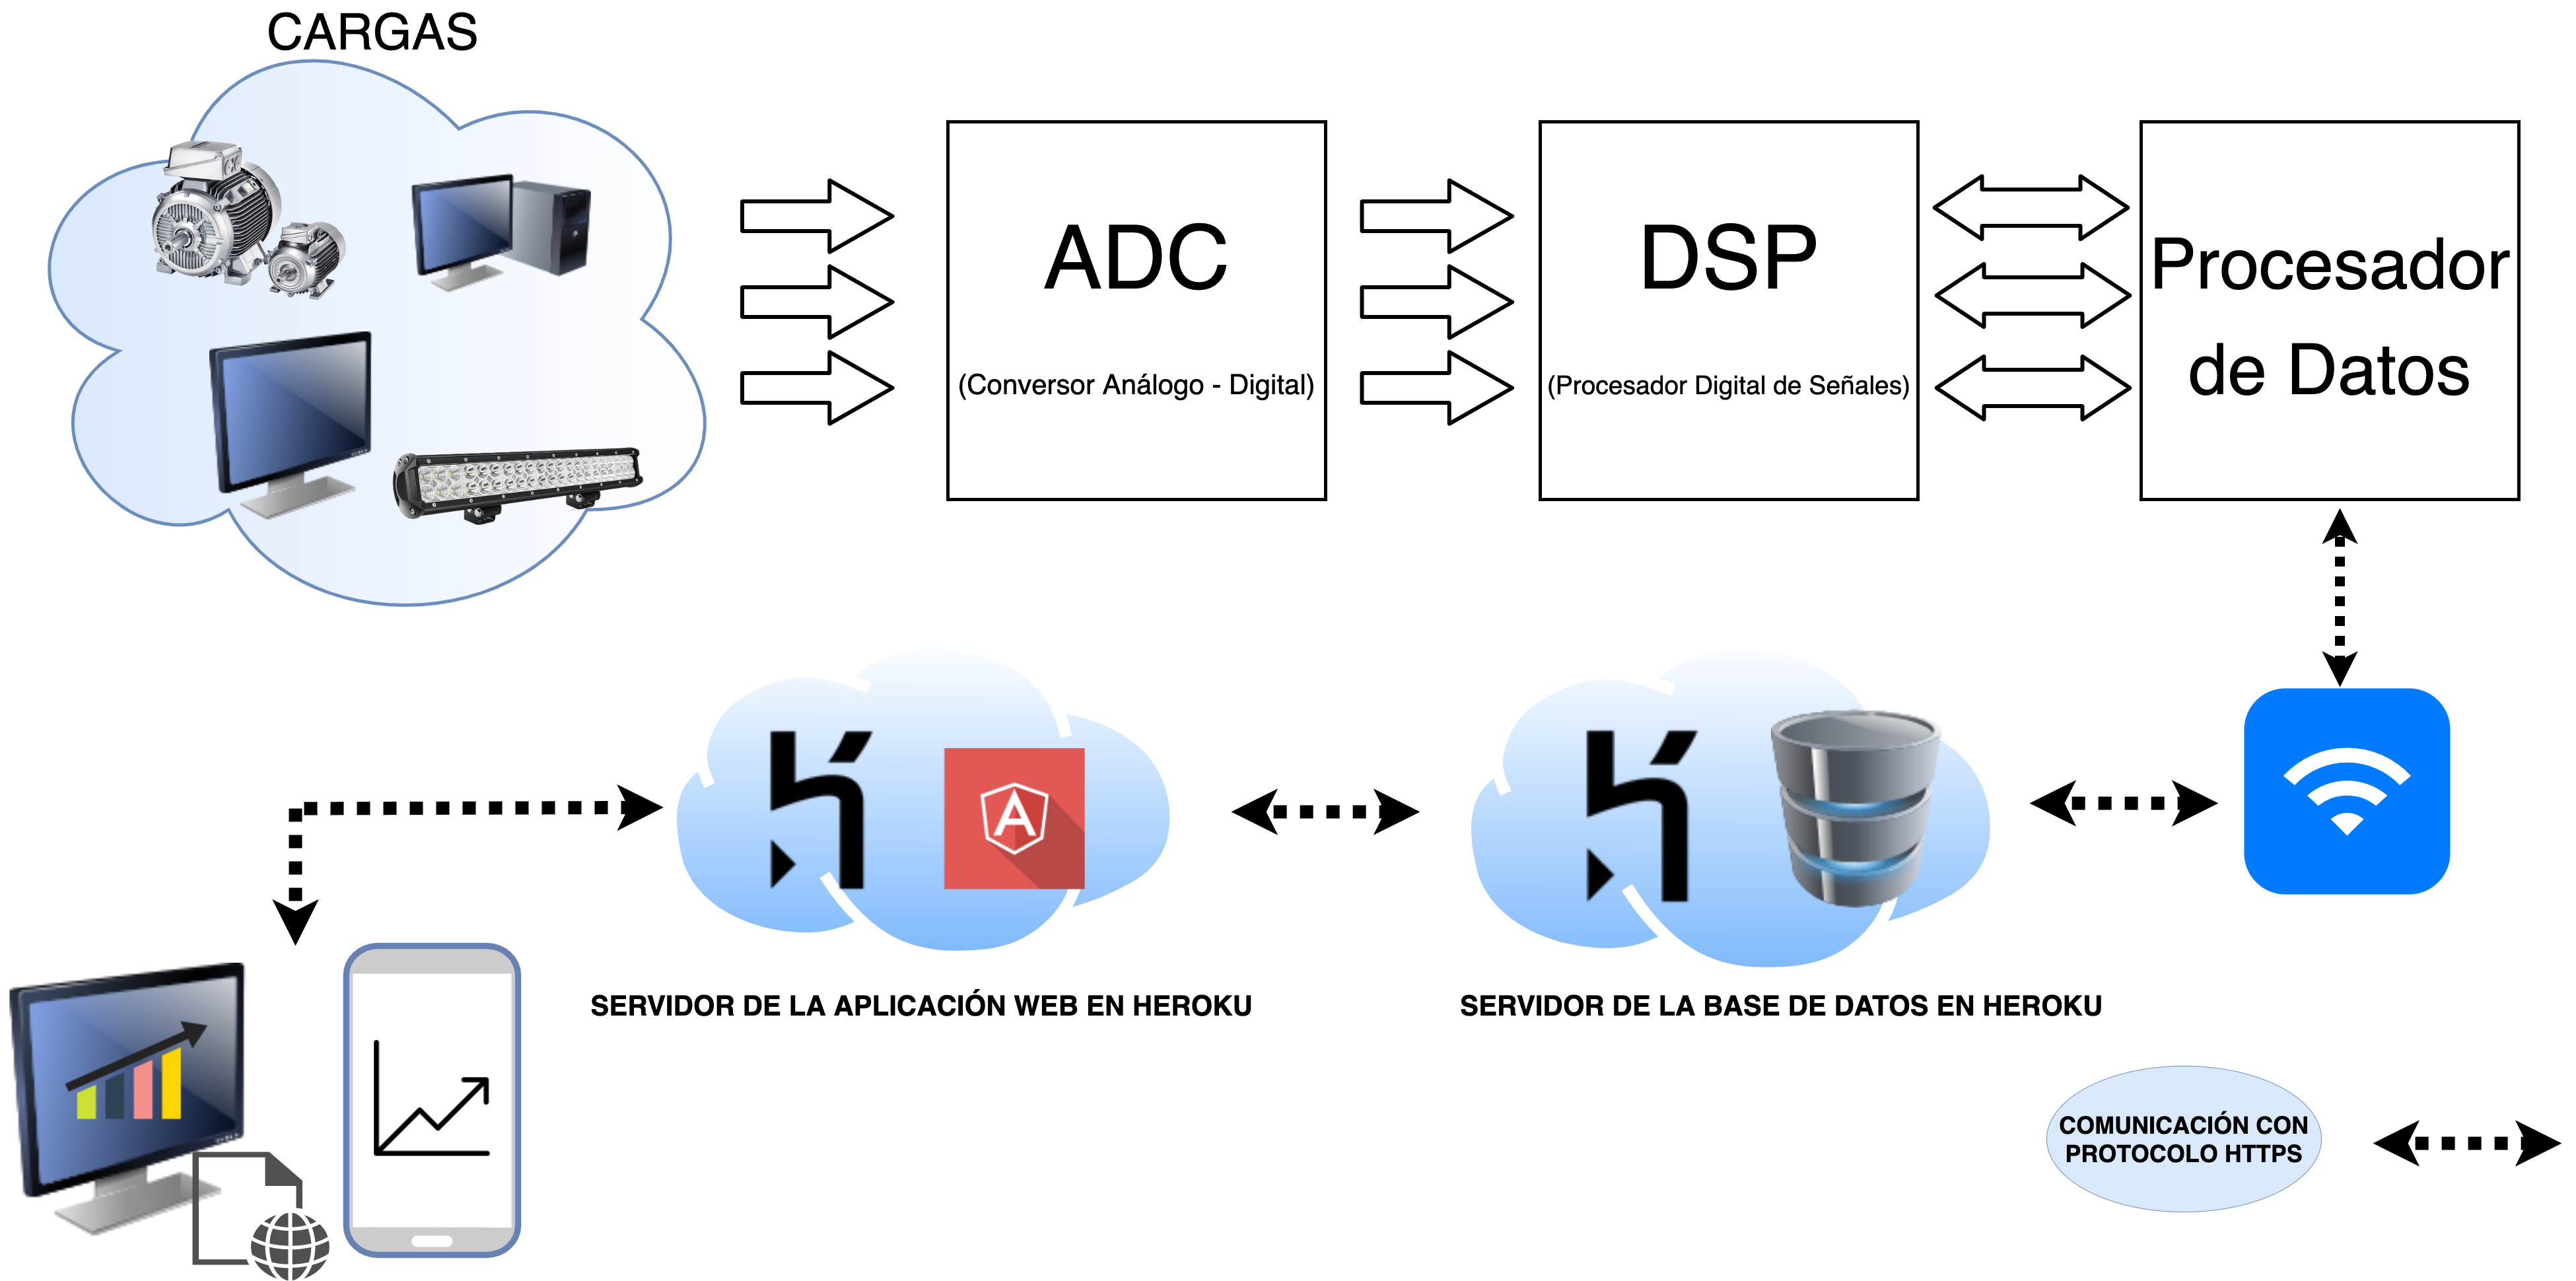
\includegraphics[width = 15cm]{3Proyecto/arquitectura}
\caption{Arquitectura del proyecto} 
\label{fig:arquitectura-proyecto}
\end{figure} 
En primera medida se planteó el diseño electrónico del medidor, iniciando por las cargas donde se conectan a un convertidor de señal análoga a digital, estas señales se pasan a un procesador digital de señales, dónde se aplica los parámetros matemáticos establecidos en el estándar IEEE 1459 del 2010, el cual da la medición de la potencia eléctrica en cualquier tipo de condición.\\\\
Dicho esto, la información se envía a un procesador de datos, este se encarga de administrar el manejo que se le da a los datos como lo es su lectura, escritura y filtración de los datos. El procesador debe contar con conexión a internet ya sea por wifi o ethernet con el fin de guardar la información en una base datos que está alojada en un servidor en la nube, la comunicación que tiene el procesador de datos con el servidor es por protocolo HTTPS.\\\\
Por lo tanto, el servidor en la nube que se planteó es Heroku ya que tiene la opción de una cuenta gratuita y así hostear la base de datos y la aplicación web sin ningún costo. Por ende las restricciones que tiene este plan, es que no se puede escoger el dominio de la página y hay un límite de espacio de 512MB pero es más que suficiente para el peso que tiene la base de datos de 21.5MB y la aplicación web de 65.2MB.\\\\
Una vez configurado el servidor, se escogió el framework javascript Angular 7 para el desarrollo de la aplicación web, ya que por medio del lenguaje de programación Typescript, el cual es un lenguaje tipado y robusto, nos permite tener mayor manipulación y consistencia en los datos; la aplicación utiliza una arquitectura RESTful y este permite, realizar peticiones HTTPS a la base de datos.\\\\
Finalmente, la información se visualiza de forma gráfica y númerica en una página web, en donde se pueden ver los valores de voltaje (V), corriente (A), potencia activa(W), potencia aparente (VA), potencia reactiva(VAR) y porcentaje de distorsión armónica en corriente y voltaje en cada fase.\\\\


\section{Fase de integración}
Considerando las fases y la magnitud del proyecto se decidió investigar e integrar un dispositivo que hiciera el análisis de las señales aplicando las ecuaciones del STD IEEE 1459 del 2010. Durante la búsqueda se encontró que los dispositivos más cercanos son los siguientes:\\
\begin{enumerate}
    \itemsep0em
    \item EVM430-F6779-3 Phase Electronic Watt-Hour EVM
    \item EVAL-ADE 7978
    \item 78M6631 3-Phase PowerMeasurement IC
\end{enumerate}

A continuación se detalla las tarjetas mencionadas:\\
\subsubsection{EVM430-F6779-3 Phase Electronic Watt-Hour EVM}
\begin{figure}
\centering
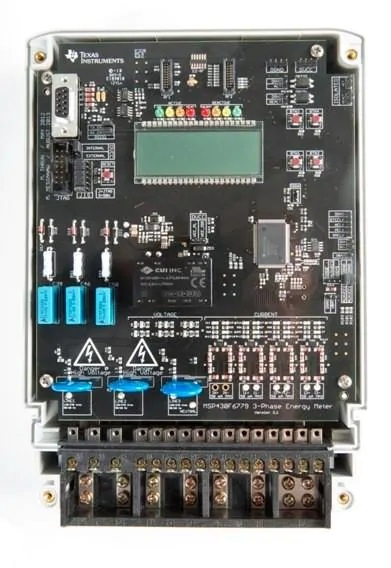
\includegraphics[width = 3cm]{3Proyecto/EVM430-F6779}
\caption{Tarjeta EVM430-F6779-3} 
\label{fig:EVM430-F6779-3}
\end{figure} 
\begin{itemize}
\itemsep0em
\item Es posible ejecutar aplicaciones de medición en tiempo real.
\item Viene con software de medición.
\item Se puede conectar a cualquier sistema de prueba o voltaje AC.
\item Fuentes de alimentación capacitaras y aisladas presentes
\item Fácil visualización de resultados y calibración a través de RS-232
\item Pantalla LCD de 160 segmentos
\item Conectores RF para soporte AMR / AMI
\item Soporte RTC de 32 kHz (cabecera disponible para calibración RTC)
\item Encabezados para alimentación MSP430 o solo  RTC a través de fuentes de alimentación auxiliares
\end{itemize}
\subsubsection{EVAL-ADE 7978}
\begin{figure}[H]
\centering
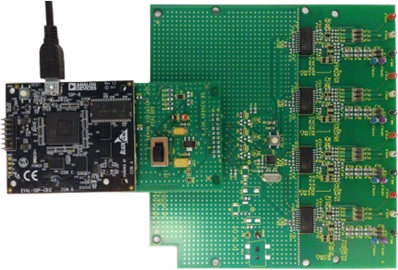
\includegraphics[width = 3cm]{3Proyecto/EVAL-ADE7978}
\caption{Tarjeta EVAL-ADE7978} 
\label{fig:EVAL-ADE7978}
\end{figure}
\begin{itemize}
\itemsep0em
\item Permite sensores Shunt en medidores de energía polifásica. 
\item Inmune a la manipulación magnética.
\item Alta precisión; admite EN 50470-1, EN 50470-3, IEC 62053-21, IEC 62053-22, IEC 62053-23, ANSI C12.20, y la estándar IEEE 1459.
\item Compatible con 3 fases, 3 o 4 lineas (Delta o estrella).
\item Calcula la energia Activa, Pasiva y Aparente en cada fase y en el sistema general.
\item Menos del 0.2\% de error en energía activa y reactiva en un rango dinámico de 2000 a 1 a TA = 25$^{\circ}$C
\item Menos del 0.1\% de error en voltaje rms en un rango dinámico de 500 a 1 a TA = 25$^{\circ}$C.
\item Menos del 0.25\% de error en corriente rms en un rango dinámico de 500 a 1 a TA = 25$^{\circ}$C.
\item Mediciones de calidad  de , incluida  la distorsión armónica total (THD).
\item Suministro de 3.3 V.
\item Temperatura de funcionamiento: -40$^{\circ}$C a +85$^{\circ}$C. 
\item Interfaces seriales flexibles I2C, SPI y HSDC.
\end{itemize}
\subsubsection{78M6631 3-Phase PowerMeasurement IC}
\begin{figure}[H]
\centering
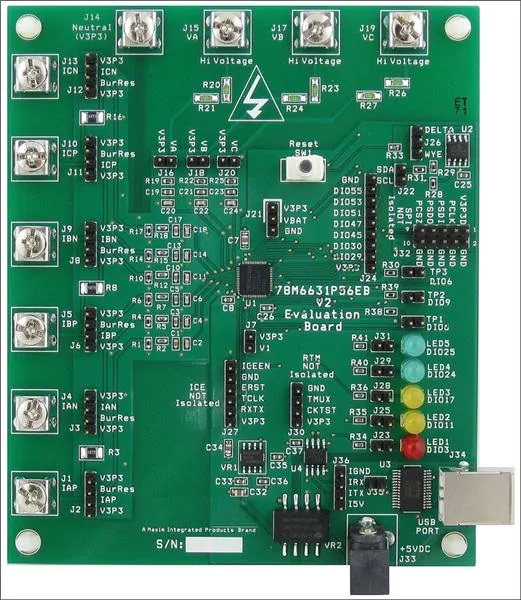
\includegraphics[width = 3cm]{3Proyecto/78M6631-EVM-DSL}
\caption{Tarjeta 78M6631-EVM-DSL}
\label{fig:78M6631-EVM-DSL}
\end{figure}
\begin{itemize}
\itemsep0em
\item 0.5 \% de precisión de vatios sobre 2000 : 1 corriente Rango y temperatura exclusiva
\item Excede los estándares IEC 62053 / ANSI C12.20.
\item Referencia de voltaje <40 ppm/ $^{\circ}$C.
\item Seis entradas analógicas que admiten entradas de medición de corriente y voltaje trifásico.
\item Configuración delta o estrella.
\item ADC Delta-Sigma de 22 bits con motor de cómputo (CE) independiente de 32 bits.
\item MPU de 8 bits (80515), un ciclo de reloj por instrucción con 4 KB MPU XRAM.
\item 128 KB Flash con seguridad.
\item Base de tiempo de 32 kHz con temporizador de vigilancia de hardware
\item Opciones de interfaz de host UART, I2C y High-Speed Slave SPI.
\item 17 pines I/O tolerante a 5V de uso general.
\end{itemize}

Teniendo encenta las características encontradas en las tres tarjetas, se decidió escoger el dispositivo ADE 7978 ya que cumple con la norma IEEE 1459 y tiene una medición precisa, ademas de esto la resolución del dispositivo es mucho mejor que el de los otros ( 24 bits ).
\section{Desarrollo del Hardware}
\subsection{Configuración inicial}

La conexión que se realizó, fue una configuración de 3 fases, 4 hilos, distribución estrella. El diagrama de conexión se ve en la figura \ref{fig:configuracion}

\begin{figure}[H]
    \begin{center}
    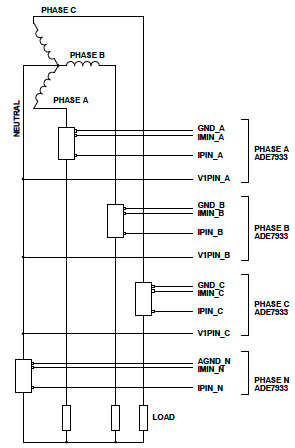
\includegraphics[width = 9cm]{3Proyecto/configuration}
    \caption{ Esquema de conexión para una distribución en Y, 3 fases, 4 hilos.} 
    \label{fig:configuracion}
    \end{center}
    \end{figure}

\subsubsection{Materiales}
\begin{itemize}
\itemsep0em
\item 4 resistencias Shunt.
\item 1m de cable 7 hilos 22 AWG azul - V1PIN.
\item 1m de cable 7 hilos 22 AWG cafe - GND.
\item 1m de cable 7 hilos 22 AWG amarillo - IMIN.
\item 1m de cable 7 hilos 22 AWG rojo - IPIN.
\item 2m de cable duplex 2x10 AWG blanco
\item 10 TYP UK2.50.
\item Carril de aluminio.
\item lamina de acetato.
\item 20 terminales.
\item 4 postes Met 10mm.
  
\end{itemize}

\begin{figure}[H]
\begin{center}
\includegraphics[width = 3cm]{3Proyecto/Cableado}
\caption{ ADE 7978 configurado con las resistencias Shunt} 
\label{fig:Cableado}
\end{center}
\end{figure}
Para configurar la tarjeta fue necesario encontrar una resistencia Shunt que se ajustará a las especificaciones del circuito a implementar, sin embargo este trabajo fue mas complicado, ya que las resistencias Shunt disponibles en el mercado son costosas y la mayoría de ellas vienen con resistencias bajas, elevando el voltaje de salida y ampliando el rango de medición del medidor ($\dfrac{I}{R}=V$), se decidió comprar 4 resistencias Shunt caseras las cuales tenían un costo de tan solo \$4.000 COP muy bajo comparado con las importadas o fabricadas industrial mente, en las que su valor esta entre \$50.000 COP - \$ 200.000 COP.\\
Teniendo todos los materiales, se realiza la conexión de la figura \ref{fig:configuracion}, utilizando el cable azul para el pin V1PIN, el cable café para el pin GND, el cable amarillo para el pin IMIN, el cable rojo para el pin IPIN y el cable blanco para conectar las shunt con el bloque de terminales, todo el montaje puesto sobre una lamina de acetato elevando la tarjeta con los 4 postes Met como se muestra en la figura \ref{fig:Cableado}\\

\subsection{Caracterización de la resistencia Shunt}
\begin{table} [H]
    \begin{center}
    \begin{tabular}{ |c|c|c|c|c|c|c|c|c| }
        \hline 
        Corriente (A) & 0.552 & 0.558 & 0.565 & 0.566 & 0.575 & 0.583 & 0.586 & 0.597\\
        \hline
        Voltaje (V) & 0.00105 & 0.00105 & 0.00107 & 0.00107 & 0.00107 & 0.00108 & 0.00109 & 0.00109\\
        \hline
        \hline 
        Corriente (A) & 0.609 & 0.621 & 0.639 & 0.651 & 0.68 & 0.7 & 0.73 & 0.757\\
        \hline
        Voltaje (V) & 0.00111 & 0.00113 & 0.00115 & 0.00117 & 0.0012 & 0.00122 & 0.00125 & 0.0013\\
        \hline
        \hline 
        Corriente (A) & 0.784 & 0.813 & 0.85 & 0.888 & 0.935 & 1.02 & 1.06 & 1.12\\
        \hline
        Voltaje (V) & 0.00134 & 0.00136 & 0.00143 & 0.00148 & 0.00153 & 0.00162 & 0.0017 & 0.00179\\
        \hline
        \hline 
        Corriente (A) & 1.21 & 1.28 & 1.38 & 1.45 & 1.59 & 1.63 & 1.75 & 1.8\\
        \hline
        Voltaje (V) & 0.0019 & 0.002 & 0.0022 & 0.00226 & 0.00246 & 0.00254 & 0.0027 & 0.00277\\
        \hline
        \hline 
        Corriente (A) & 1.75 & 1.67 & 1.5 & 1.42 & 1.35 & 1.24 & 1.18 & 1.1\\
        \hline
        Voltaje (V) & 0.00269 & 0.00257 & 0.00233 & 0.00222 & 0.00211 & 0.00196 & 0.00187 & 0.00176\\
        \hline
        \hline 
        Corriente (A) & 1.06 & 1.01 & 0.97 & 0.92 & 0.879 & 0.84 & 0.816 & 0.777\\
        \hline
        Voltaje (V) & 0.00169 & 0.00163 & 0.00158 & 0.00151 & 0.00145 & 0.0014 & 0.00137 & 0.00131\\
        \hline
        \hline 
        Corriente (A) & 0.753 & 0.734 & 0.71 & 0.693 & 0.67 & 0.652 & 0.629 & 0.616\\
        \hline
        Voltaje (V) & 0.00127 & 0.00125 & 0.00122 & 0.00119 & 0.00116 & 0.00115 & 0.00112 & 0.00111\\
        \hline
        \hline
        Corriente (A) & 0.605 & 0.591 & 0.575 & 0.562 & 0.555 \\
        \hline
        Voltaje (V) & 0.0011 & 0.00108 & 0.00107 & 0.00105 & 0.00104 \\ 
        \hline
    \end{tabular}
\end{center}
\caption{Corriente vs Voltaje en la resistencia shunt A}
\label{tab:shuntA}
\end{table}

\begin{figure}[H]
    \begin{center}
    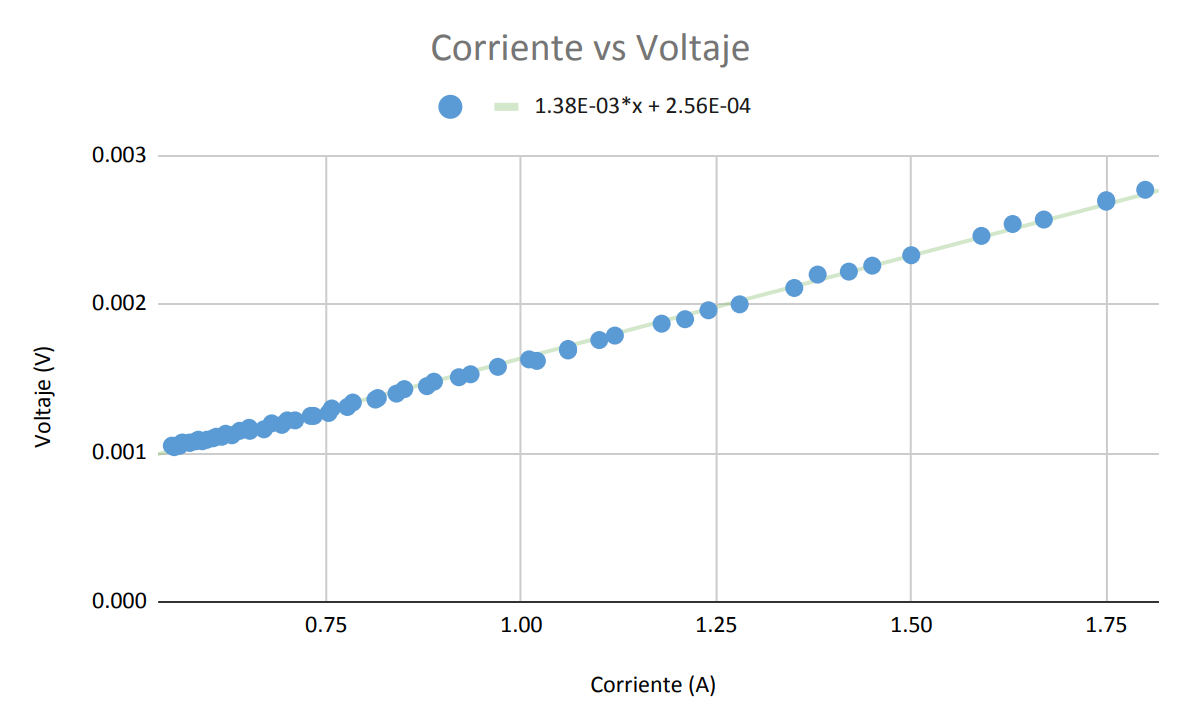
\includegraphics[width = 15cm]{3Proyecto/CorrienteVoltaje1.png}
    \caption{ Caracterización ShuntA} 
    \label{fig:Muestras ShuntA}
    \end{center}
\end{figure}




\begin{table} [H]
    \begin{center}
    \begin{tabular}{ |c|c|c|c|c|c|c|c|c| }
        \hline
        Corriente (A) & 0.549 & 0.574 & 0.606 & 0.633 & 0.67 & 0.698 & 0.744 & 0.77\\
        \hline
        Voltaje (V) & 0.00107 & 0.00111 & 0.00112 & 0.00115 & 0.00119 & 0.00125 & 0.0013 & 0.00133\\
        \hline
        \hline
        Corriente (A) & 0.823 & 0.867 & 0.922 & 0.99 & 1.05 & 1.15 & 1.23 & 1.36\\
        \hline
        Voltaje (V) & 0.0014 & 0.00145 & 0.00152 & 0.0016 & 0.0017 & 0.00186 & 0.00196 & 0.00213\\
        \hline
        \hline
        Corriente (A) & 1.48 & 1.69 & 1.8 & 1.7 & 1.48 & 1.35 & 1.22 & 1.15\\
        \hline
        Voltaje (V) & 0.0023 & 0.0026 & 0.00278 & 0.00262 & 0.0023 & 0.00214 & 0.00194 & 0.00182\\
        \hline
        \hline
        Corriente (A) & 1.05 & 0.977 & 0.913 & 0.85 & 0.811 & 0.76 & 0.728 & 0.685\\
        \hline
        Voltaje (V) & 0.0017 & 0.00162 & 0.00151 & 0.00143 & 0.00139 & 0.00132 & 0.00127 & 0.0012\\
        \hline
        \hline
        Corriente (A) & 0.662 & 0.635 & 0.611 & 0.599 & 0.58 & 0.557\\
        \hline
        Voltaje (V) & 0.00119 & 0.00116 & 0.00113 & 0.0011 & 0.00109 & 0.00108\\
        \hline
    \end{tabular}
\end{center}
\caption{Corriente vs Voltaje en la resistencia shunt B}
\label{tab:shuntB}
\end{table}
\begin{figure}[H]
    \begin{center}
    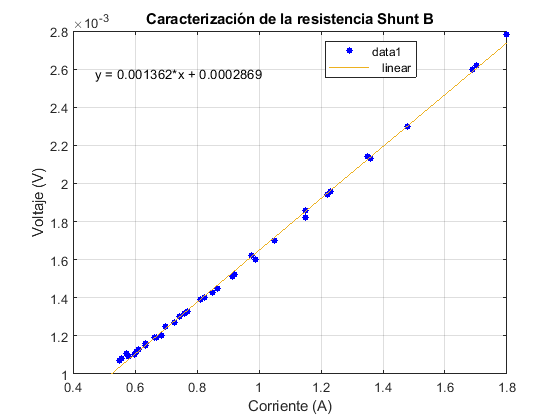
\includegraphics[width = 15cm]{3Proyecto/CorrienteVoltaje2.png}
    \caption{ Caracterización ShuntB} 
    \label{fig:Muestras shuntB}
    \end{center}
\end{figure}



\begin{table} [H]
    \begin{center}
    \begin{tabular}{ |c|c|c|c|c|c|c|c|c| }
        \hline
        Corriente (A) & 0.557 & 0.573 & 0.593 & 0.631 & 0.654 & 0.69 & 0.717 & 0.752\\
        \hline
        Voltaje (V) & 0.00106 & 0.00108 & 0.0011 & 0.00115 & 0.00117 & 0.00122 & 0.00126 & 0.00131\\
        \hline
        \hline
        Corriente (A) & 0.8 & 0.838 & 0.896 & 0.95 & 1.03 & 1.09 & 1.19 & 1.29\\
        \hline
        Voltaje (V) & 0.00137 & 0.00141 & 0.00149 & 0.00155 & 0.00166 & 0.00175 & 0.00189 & 0.00205\\
        \hline
        \hline
        Corriente (A) & 1.47 & 1.59 & 1.8 & 1.63 & 1.52 & 1.37 & 1.27 & 1.15\\
        \hline
        Voltaje (V) & 0.0023 & 0.00246 & 0.00276 & 0.00251 & 0.00237 & 0.00215 & 0.00199 & 0.00183\\
        \hline
        \hline
        Corriente (A) & 1.07 & 0.98 & 0.925 & 0.86 & 0.816 & 0.766 & 0.737 & 0.697\\
        \hline
        Voltaje (V) & 0.00172 & 0.0016 & 0.00153 & 0.00144 & 0.00138 & 0.00131 & 0.0013 & 0.00121\\
        \hline
        \hline
        Corriente (A) & 0.661 & 0.633 & 0.616 & 0.599 & 0.558\\
        \hline
        Voltaje (V) & 0.00119 & 0.00115 & 0.00113 & 0.00111 & 0.00107\\
        \hline
    \end{tabular}
\end{center}
\caption{Corriente vs Voltaje en la resistencia shunt C}
\label{tab:shuntC}
\end{table}

\begin{figure}[H]
    \begin{center}
    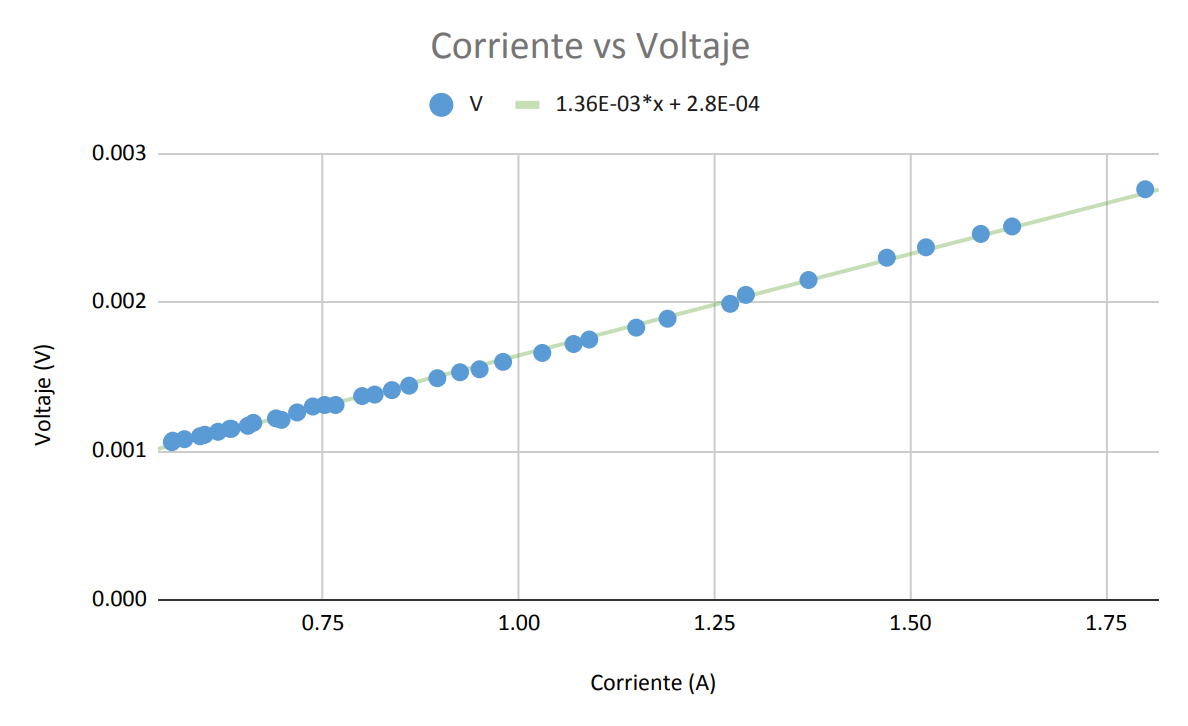
\includegraphics[width = 15cm]{3Proyecto/CorrienteVoltaje3.png}
    \caption{ Caracterización ShuntC} 
    \label{fig:Muestras shuntC}
    \end{center}
\end{figure}


\subsection{Conversión de voltaje}
Para obtener el voltaje de entrada del ADE7978, se realizaron los siguientes pasos:\\

La carga se conecta a la fase siguiendo el diagrama de conexión \ref{fig:configuracion}. Los pines V1PIN y GND\_A, pasan por un divisor de voltaje donde su salida es el pin V1P y VM como se ve en la figura \ref{fig:divisorVolate}. El divisor se modela bajo la siguiente ecuación:\\

\begin{equation}
    V1P = \frac{R_{2}}{R_{1} + R_{2}} * V_{in}
\end{equation}

Donde $\; R1 = 990150 \ohm$, \;$R2 = 1 K\ohm$.\\

\begin{equation}\label{divisorVoltaje}
    V1P = 0.00100893 * V_{in}
\end{equation}

El divisor de voltaje es necesario ya que el conversor ADE7933 solo debe recibir valores en un rango de $\pm 0.5V$. 

El voltaje VA es la diferencia de voltaje que hay entre V1P y VM, esta es la señal que el conversor transforma a digital. La salida digital que entrega el conversor tiene un rango de $\pm 5.320.000$ como se ve en la figura \ref{fig:voltageOutput}. Esta señal entra al ADE7978 y de ahí en adelante, todos los procesos que se ejecutan, son basados en la conversión anteriormente descrita.\\

La relación de entrada y salida del conversor ADE7933, consiste en un voltaje pico de entrada de $0.5 V$, genera una señal de salida de $5.320.000$.\\

La siguiente ecuación relaciona la señal de salida del conversor con la señal de entrada al medidor:\\

\begin{align*}
    &0,5V \rightarrow 5,320,000.\\
    &V1P \rightarrow DRV
\end{align*}

Donde $DRV = Dato\;del\;rango\;de\;voltaje\;del\;conversor$\\

\begin{equation}
    V1P = \frac{DRV * 0.5}{5.320.000}
\end{equation}

\begin{equation}\label{relacionConversor}
    V1P = DRV * 9,39845 * 10^{-8} 
\end{equation}

Reemplazando la ecuación del divisor de voltaje \ref{divisorVoltaje} en \ref{relacionConversor}

\begin{align*}
    0.00100893 * V_{in} = DRV * 9,39845 * 10^{-8} 
\end{align*}

\begin{equation}\label{conversorEntradaSalida}
    V_{in} = DRV * 0,00009315311
\end{equation}
La ecuación \ref{conversorEntradaSalida} modela la relación del voltaje de entrada al circuito al rango de voltaje del conversor.

\begin{figure}[H]
    \centering
    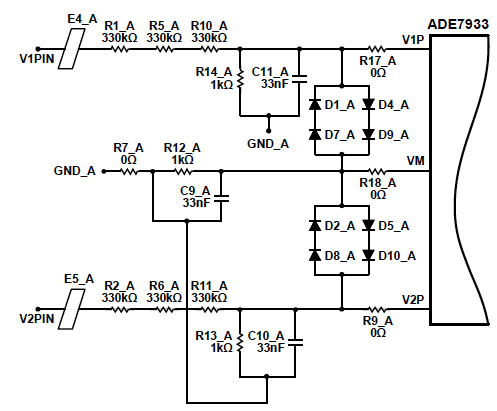
\includegraphics[width = 10cm]{3Proyecto/divisorVoltaje}
    \caption{Divisor de voltaje ADC} 
    \label{fig:divisorVolate}
\end{figure} 

\begin{figure}[H]
    \centering
    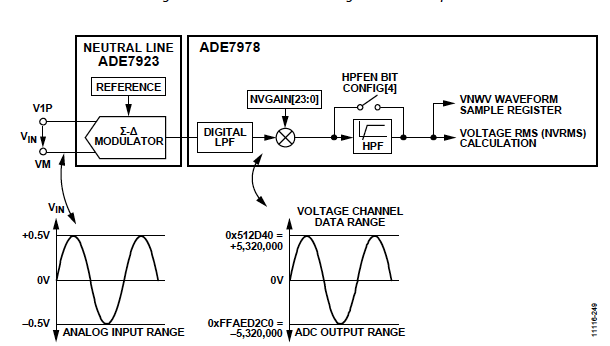
\includegraphics[width = 10cm]{3Proyecto/voltageOutput}
    \caption{Salida de voltaje del ADE 7978} 
    \label{fig:voltageOutput}
\end{figure} 


\subsection{Conversión de corriente}
Para encontrar la relación que hay entre la entrada de corriente y el convertidor ADC fue necesario utilizar la ecuación de la recta arrojada por las muestras de la caracterización de las shunt y también fue necesario hallar la relación de voltaje entre el pin IP e IM que son los usados por el ADC figura \ref{fig:CircuitoCorriente}


\begin{figure}[H]
    \begin{center}
        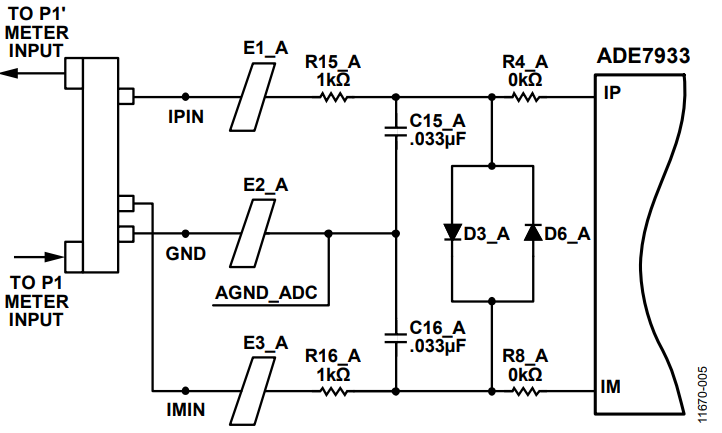
\includegraphics[width = 10cm]{3Proyecto/CircuitoCorriente.PNG}
    \caption{ Circuito de protección para los pines IP e IM } 
    \label{fig:CircuitoCorriente}
   \end{center}
\end{figure}

Como ya se tiene la relación entre la corriente de entrada y el voltaje de salida en la Shunt se procede hallar el voltaje entre el pin IP e IM resolviendo el circuito por medio del teorema de nodos como se muestra en la figura \ref{fig:Nodos}
\begin{figure}[H]
    \begin{center}
        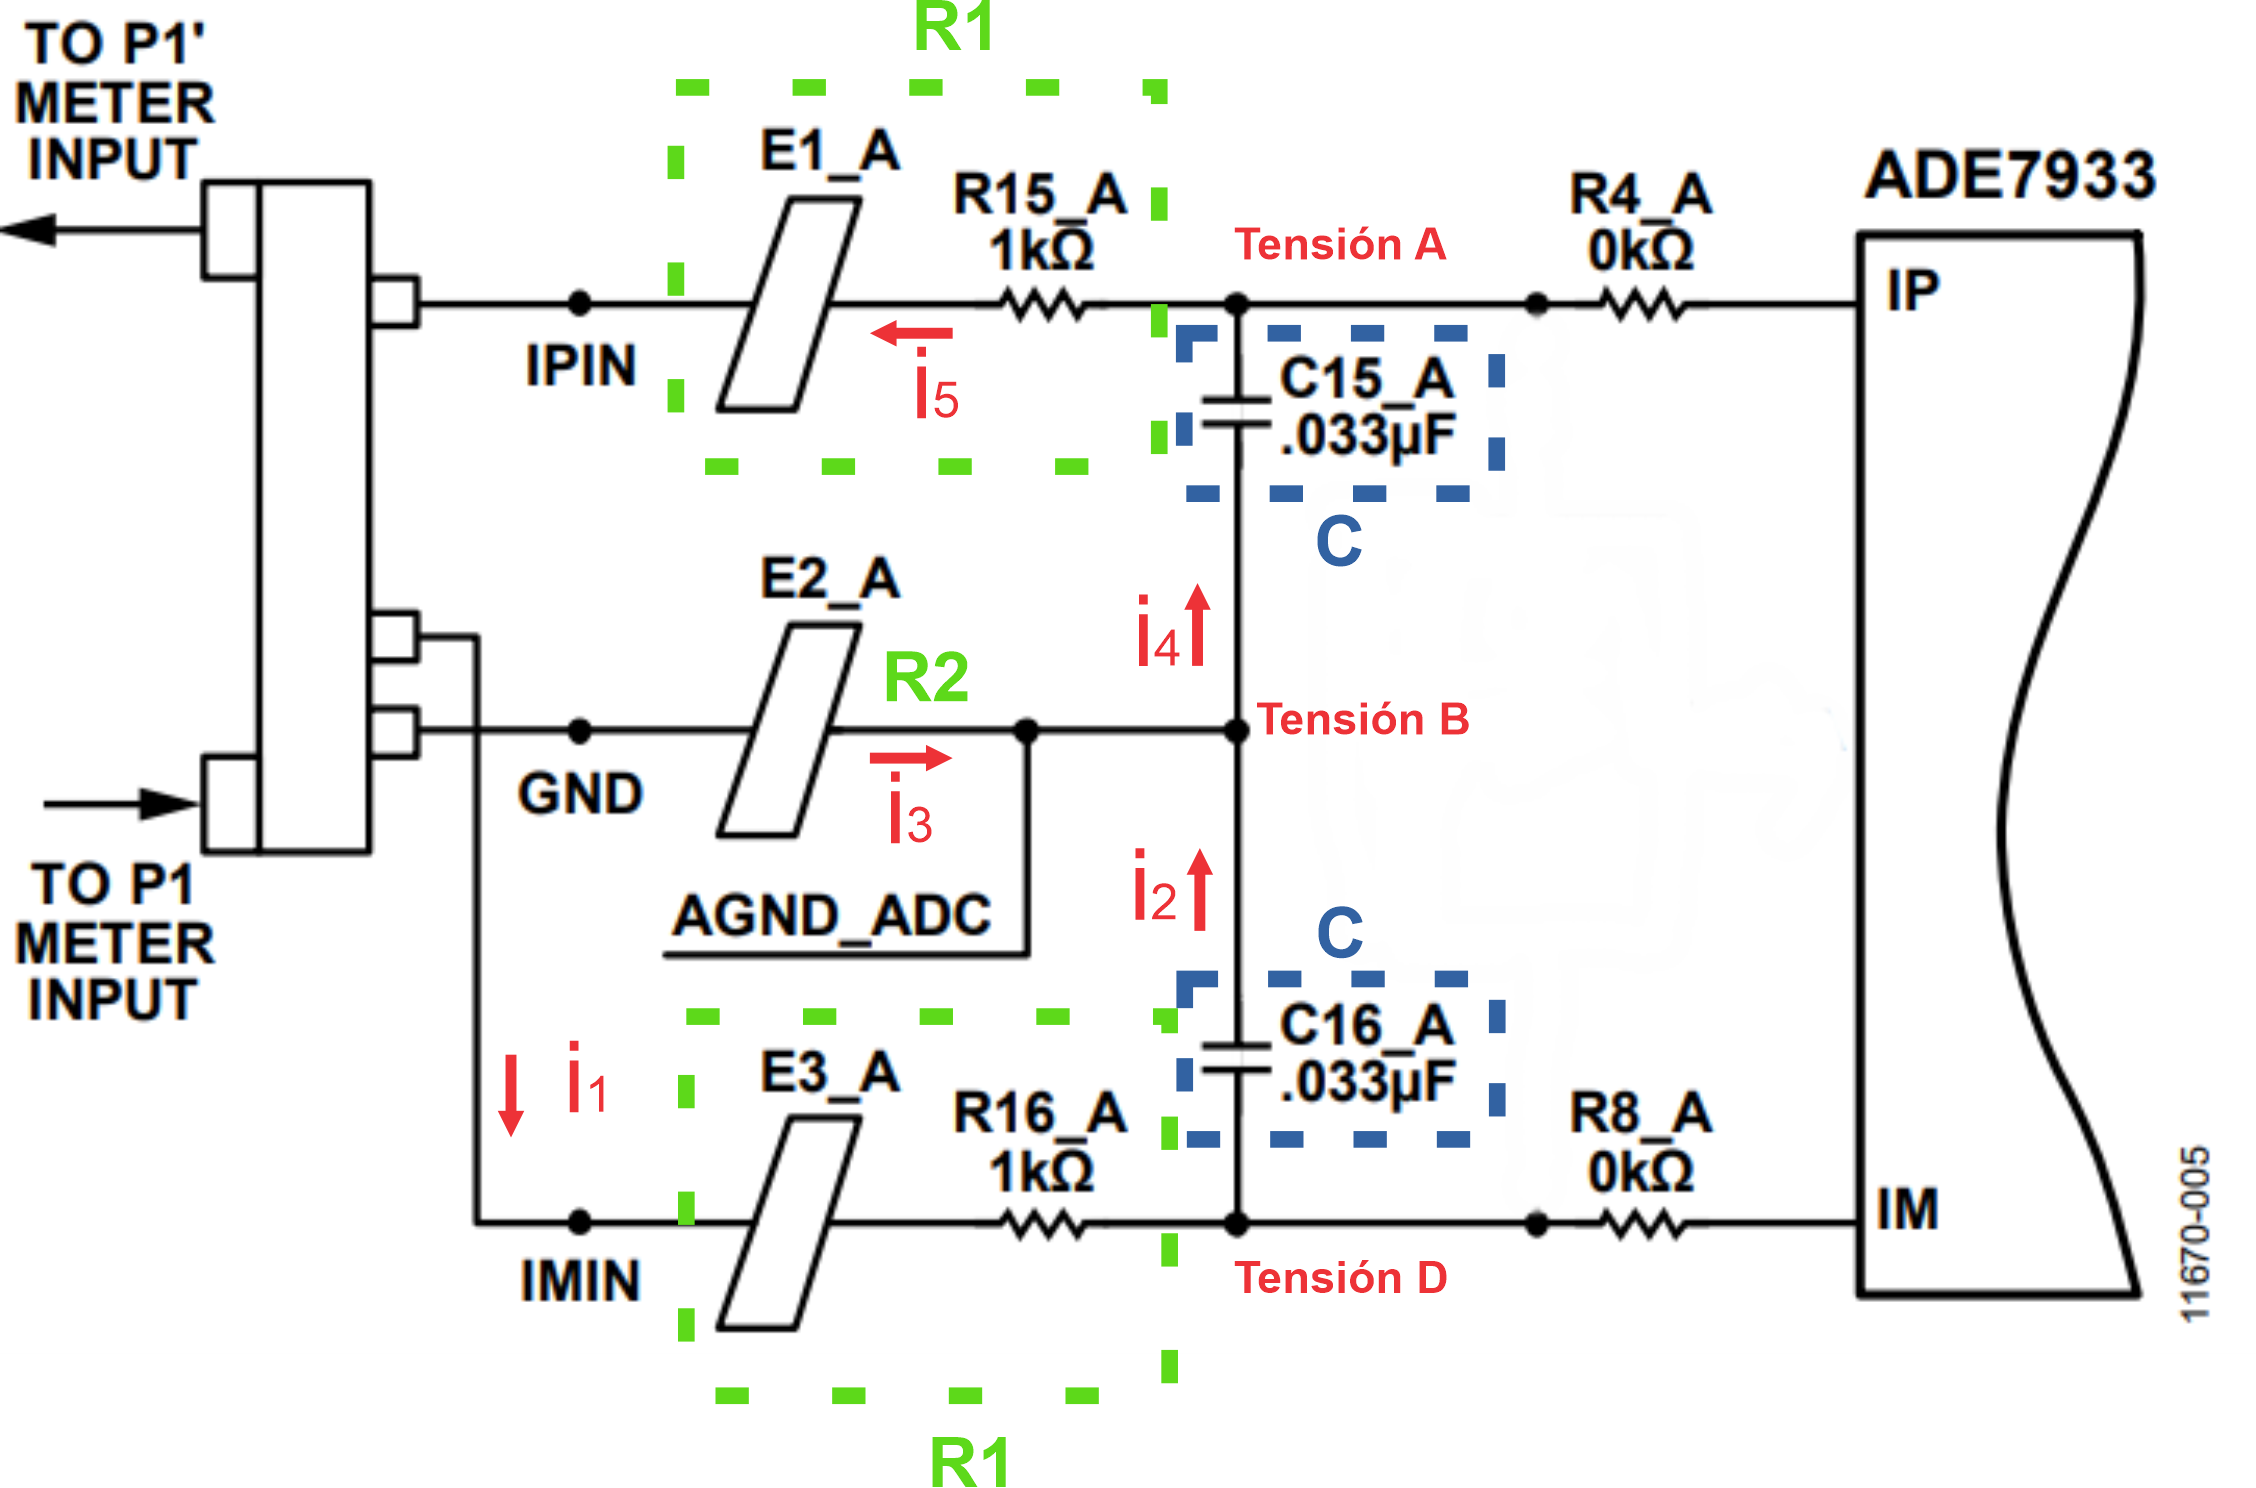
\includegraphics[width = 10cm]{3Proyecto/Nodos.PNG}
    \caption{ Nodos aplicados al circuito} 
    \label{fig:Nodos}
   \end{center}
\end{figure}

Se asume que el circuito se alimenta con una fuente de voltaje AC con terminal $+$ en IPIN y terminal $-$ en GND e IMIN resolviendo de la siguiente manera :
\\  
\begin{equation}\label{Nodo D}
\end{equation}

Con las ecuaciones obtenidas de cada nodo se despeja cada una de ellas dejándola igualada a una variable 
\begin{itemize}
    \item \textbf{Nodo A} \\
    $\mathbf{i_{1}=i_{2}}$
    \begin{align*}
        \frac{V_{i}}{R_{1}} - \frac{A}{R_{1}} = \frac{A}{ZC} - \frac{B}{ZC} \\\\
        \frac{V_{i}}{R_{1}} = A(\frac{1}{R_{1}}+\frac{1}{ZC}) -\frac{B}{ZC} \\\\
        \frac{V_{i}}{R_{1}} = A\frac{R_{1}+ZC}{R_{1}ZC} -\frac{B}{ZC} \\\\
            \frac{B}{ZC} = A\frac{R_{1}+ZC}{R_{1}ZC} - \frac{V_{i}}{R_{1}}
        \end{align*}
        \begin{equation}\label{Nodo A}
            B = A\frac{R_{1}+ZC}{R_{1}} - V_{i}\frac{ZC}{R_{1}}
        \end{equation}
        \item \textbf{Nodo B} \\
        $ \mathbf{i_{2}=i_{3}+i_{4}}$
        \begin{align*}
            \frac{A}{ZC} - \frac{B}{ZC} = \frac{B}{R_{2}} + \frac{B}{ZC} - \frac{D}{ZC} \\\\
            \frac{A}{ZC} + \frac{D}{ZC} = B(\frac{1}{R_{2}} + \frac{1}{ZC} + \frac{1}{ZC}) \\\\
            \frac{A}{ZC} + \frac{D}{ZC} = B(\frac{1}{R_{2}} + \frac{2}{ZC} ) \\\\
            \frac{A}{ZC} + \frac{D}{ZC} = B\frac{2R_{2}+ZC}{R_{2}ZC} 
        \end{align*}
        \begin{equation}\label{Nodo B}
            B = A\frac{R_{2}}{2R_{2}+ZC} + D\frac{R_{2}}{2R_{2}+ZC}
        \end{equation}
        \item \textbf{Nodo D} \\
        $ \mathbf{i_{4}=i_{5}}$
        \begin{align*}
            \frac{B}{ZC} - \frac{D}{ZC} = \frac{D}{R_{3}} \\\\
            \frac{B}{ZC} = D(\frac{1}{R_{3}} + \frac{1}{ZC}) \\\\
            \frac{B}{ZC} = D\frac{R_{3}+ZC}{R_{3}ZC}
        \end{align*}
        \begin{equation}\label{Nodo D}
            B = D\frac{R_{3}+ZC}{R_{3}}
        \end{equation}
    \end{itemize}
    
    Remplazando la ecuación \ref{Nodo B} en la ecuación \ref{Nodo A}
    \begin{align*}
        A\frac{R_{2}}{2R_{2}+ZC} + D\frac{R_{2}}{2R_{2}+ZC} = A\frac{R_{1}+ZC}{R_{1}} - V_{i}\frac{ZC}{R_{1}} \\\\
        D\frac{R_{2}}{2R_{2}+ZC} = A(\frac{R_{1}+ZC}{R_{1}} - \frac{R_{2}}{2R_{2}+ZC})- V_{i}\frac{ZC}{R_{1}} \\\\
        D\frac{R_{2}}{2R_{2}+ZC} = A\frac{(R_{1}+ZC)(2R_{2}+ZC) - R_{1}R_{2}}{R_{1}(2R_{2}+ZC)} - V_{i}\frac{ZC}{R_{1}} \\\\
        D = A\frac{((R_{1}+ZC)(2R_{2}+ZC) - R_{1}R_{2})(2R_{2}+ZC)}{R_{1}R_{2}(2R_{2}+ZC)} - V_{i}\frac{ZC(2R_{2}+ZC)}{R_{1}R_{2}}
    \end{align*}
    \begin{equation}\label{Nodo B en A}
        D = A\frac{(R_{1}+ZC)(2R_{2}+ZC) - R_{1}R_{2}}{R_{1}R_{2}} - V_{i}\frac{ZC(2R_{2}+ZC)}{R_{1}R_{2}}
    \end{equation}
    
    Remplazando la ecuación \ref{Nodo B} en la ecuación \ref{Nodo D}
    \begin{align*}
        A\frac{R_{2}}{2R_{2}+ZC} + D\frac{R_{2}}{2R_{2}+ZC} = D\frac{R_{3}+ZC}{R_{3}} \\\\
        A\frac{R_{2}}{2R_{2}+ZC} = D(\frac{R_{3}+ZC}{R_{3}}-\frac{R_{2}}{2R_{2}+ZC}) \\\\
        A\frac{R_{2}}{2R_{2}+ZC} = D(\frac{(2R_{2}+ZC)(R_{3}+ZC)-R_{2}R_{3}}{R_{3}(2R_{2}+ZC)} \\\\
        AR_{2} = D(\frac{(2R_{2}+ZC)(R_{3}+ZC)-R_{2}R_{3}}{R_{3}}
    \end{align*}
    \begin{equation}\label{Nodo B en D}
        A\frac{R_{2}R_{3}}{(2R_{2}+ZC)(R_{3}+ZC)-R_{2}R_{3}} = D 
    \end{equation}
    
    Remplazando la ecuación \ref{Nodo B en D} en la ecuación \ref{Nodo B en A}
    \begin{align*}
        A\frac{R_{2}R_{3}}{(2R_{2}+ZC)(R_{3}+ZC)-R_{2}R_{3}} = A\frac{(R_{1}+ZC)(2R_{2}+ZC) - R_{1}R_{2}}{R_{1}R_{2}} - V_{i}\frac{ZC(2R_{2}+ZC)}{R_{1}R_{2}}\\\\ 
        V_{i}\frac{ZC(2R_{2}+ZC)}{R_{1}R_{2}} = A\frac{(R_{1}+ZC)(2R_{2}+ZC) - R_{1}R_{2}}{R_{1}R_{2}} - A\frac{R_{2}R_{3}}{(2R_{2}+ZC)(R_{3}+ZC)-R_{2}R_{3}} \\\\ 
        V_{i}\frac{ZC(2R_{2}+ZC)}{R_{1}R_{2}} = A(\frac{(R_{1}+ZC)(2R_{2}+ZC) - R_{1}R_{2}}{R_{1}R_{2}} - \frac{R_{2}R_{3}}{(2R_{2}+ZC)(R_{3}+ZC)-R_{2}R_{3}}) \\\\ 
        V_{i}\frac{ZC(2R_{2}+ZC)}{R_{1}R_{2}} = A\frac{ [(R_{1}+ZC)(2R_{2}+ZC) - R_{1}R_{2}] [(2R_{2}+ZC)(R_{3}+ZC) - R_{2}R_{3}] - R_{1}R_{2}^{2}R_{3}}{(R_{1}R_{2})((2R_{2}+ZC)(R_{3}+ZC)-R_{2}R_{3})} \\\\ 
        V_{i}ZC(2R_{2}+ZC) = A\frac{ [(R_{1}+ZC)(2R_{2}+ZC) - R_{1}R_{2}] [(2R_{2}+ZC)(R_{3}+ZC)-R_{2}R_{3}] - R_{1}R_{2}^{2}R_{3} }{ (2R_{2}+ZC)(R_{3}+ZC)-R_{2}R_{3} } \\\\ 
        V_{i}\frac{ [ZC(2R_{2}+ZC)] [(2R_{2}+ZC)(R_{3}+ZC)-R_{2}R_{3}] }{ [(R_{1}+ZC)(2R_{2}+ZC) - R_{1}R_{2}] [(2R_{2}+ZC)(R_{3}+ZC)-R_{2}R_{3}]-R_{1}R_{2}^{2}R_{3} } = A\\\\ 
    \end{align*}
    Con ayuda del software Matlab se simplifica la expresión remplazando los valores de cada elemento como se muestra en el datasheet
    \\
    $ R_{1} = 1150 \ohm;$ $R_{2} = 150 \ohm;$ $R_{3} = 1150 \ohm;$ $ZC = \frac{-j}{WC};$
    $W = 2 \pi f;$ $f = 60 Hz;$ $C = 0.033\mu f ;$
    \begin{equation}\label{final A}
        V_{i}(0.9998 - 0.0143j)=A
    \end{equation}
    Magnitud = 0.9999 \\
    Angulo = -0.0143 $^{\circ}$ \\
    Remplazando la ecuación \ref{final A} en la ecuación \ref{Nodo B en A} para encontrar el valor del nodo D
    \begin{align*}
        D = A\frac{(R_{1}+ZC)(2R_{2}+ZC) - R_{1}R_{2}}{R_{1}R_{2}} - V_{i}\frac{ZC(2R_{2}+ZC)}{R_{1}R_{2}}\\\\
        D = [V_{i}(0.9998 - 0.0143j)] [\frac{(R_{1}+ZC)(2R_{2}+ZC) - R_{1}R_{2}}{R_{1}R_{2}}] - V_{i}\frac{ZC(2R_{2}+ZC)}{R_{1}R_{2}}\\\\
        D = [V_{i}(0.9998 - 0.0143j)] [-3.7455e^{4} - 6.7567e^{2}j] - V_{i}(-3.7456e^{4} - 1.3979e^{2}j)\\\\
        D = V_{i} (-2.6677e^{-5} + 8.6311e^{-7}j) \\\\
    \end{align*}
    
    La relación que hay entre el pin IP e IM es la resta entre el nodo A y e nodo D
    
    \begin{align*}
        A-D = IP-IM\\\\
        V_{i}(0.9998 - 0.0143j) - V_{i} (-2.6677e^{-5} + 8.6311e^{-7}j) = IP-IM\\\\
        V_{i}(0.9998 - 0.0143j) = IP-IM \\
        V_{i} (0.9999 \angle -0.0143) =  IP-IM
    \end{align*}
    Usando la relación arrojada en la caracterización de las resistencias, se remplaza en esta ecuación para dejar la expresión en términos de corriente de entrada en la Shunt y voltaje entre el pin IP e IM\\\\
    \begin{align*}
        &1.38e^{-3} I + 2.56e^{-4} = V_{i}\\\\
    \end{align*}
    \begin{equation}\label{Relacion corriente}
        (1.38e^{-3} I + 2.56e^{-4})(0.9999 \angle -0.0143)  = IP-IM
    \end{equation}
    La siguiente ecuación relaciona la señal de salida del conversor con la señal de entrada al medidor:\\

    \begin{align*}
        &0.03125V \rightarrow 5,320,000.\\
        &IP-IM \rightarrow DRI
    \end{align*}
    
    Donde $DRI = Dato\;del\;rango\;de\;corriente\;del\;conversor$\\
    
    \begin{equation}\label{Relacion DRI}
        IP-IM = \frac{DRI * 0.03125}{5.320.000}
    \end{equation}
    
    Remplazando la ecuación \ref{Relacion corriente} en la ecuación \ref{Relacion DRI}
    \begin{align*}
        (1.38e^{-3} I + 2.56e^{-4})(0.9998 - 0.0143j) = \frac{DRI * 0.03125}{5.320.000} \\\\
        (0.0014 - 0.0000j)I + (2.5595e^{-4} - 3.6618e^{-6}j)  = \frac{DRI * 0.03125}{5.320.000} \\\\
        I = \frac{\frac{DRI * 0.03125}{5.320.000} - (2.5595e^{-4} - 3.6618e^{-6}j)}{(0.0014 - 0.0000j)}  \\\\
        I = DRI (4.2566e^{-6} + 6.0898e^{-8}j) - (0.1855 - 0.0000j)   \\\\
        I = 4.2570e^{-6}DRI  - 0.1855   \\\\
    \end{align*}


    \section{Desarrollo de Software}

    \subsection{Implementación del protocolo I2C entre la rasberry y el ADE7978}

    \subsection{Backend Solución en c++}
    \subsection{Backend Configuración del servidor}

    Se realizó una investagación de servidores en la nube y optamos por usar Heroku ya que tiene una opción gratuita que permite hostear hasta 5 aplicaiones con un límite de peso de 512MB. \\

    \subsubsection{Configuración de la base de datos}
    
    Para realizar la configuración de la base de datos en Heroku, se hizo atravez del gestor de paquetes de javascript Node Js. En las instruccions del package.json se ejecuta el comando npm run start el cual ejecuta un archivo javascript con el siguiente código:\\

    \begin{lstlisting}
        const jsonServer = require('json-server');
        const server = jsonServer.create();
        const router = jsonServer.router('db.json');
        const middlewares = jsonServer.defaults();
        const port = process.env.PORT || 3000;

        server.use(middlewares);
        server.use(router);

        server.listen(port);
        \end{lstlisting}
    De esta manera, Node levanta un servidor local en el puerto 3000 y heroku lo expone publicamente atravez de la URL https://json-ade-metering.herokuapp.com/.

    \subsubsection{Configuración de la aplicación en Angilar 7}

    La configurac

    
    \subsection{Backend Solución con Node.js}


    \subsection{Frontend Solución en Angular}
    hola otra vez